\section{Задание №1 (Вариант 51)}\label{01-lab}

\subsection{Условие}\label{01-lab-condition}

Найти решение задачи линейного программирования геометрически.

\[
    F(x_1, x_2) = 3x_1 + x_2 \to \max(\min)\\
\]

\[
    {\huge{\text{а).}\ }}
    \begin{cases}
        2x_1 + x_2 \leq 2  \\
        -x_1 + 3x_2 \leq 3 \\
        x_1 \geq 0         \\
        x_2 \geq 0
    \end{cases}
    \hspace{1.5cm}
    {\huge{\text{б).}\ }}
    \begin{cases}
        x_1 - 3x_2 \leq 2 \\
        x_1 + x_2 \geq 10 \\
        x_1 \geq 0        \\
        x_2 \geq 0
    \end{cases}
    \hspace{1.5cm}
    {\huge{\text{в).}\ }}
    \begin{cases}
        -x_1 + x_2 \geq 11 \\
        x_1 - 4x_2 \geq 8  \\
        x_1 \geq 0         \\
        x_2 \geq 0
    \end{cases}
\]

\subsection{Решение}\label{01-lab-solution}

Для всех пунктов нам понадобится знать вектор градиента функции $F(x_1, x_2)$.

\[\overrightarrow{grad}F(x_1, x_2) = \left\{\deriv{F}{x_1}(x_1, x_2), \deriv{F}{x_2}(x_1, x_2)\right\} = \left\{3, 1\right\}\]

\subsubsection{Пункт А}\label{01-lab-a}

Приведем неравенство к более наглядному виду, чтобы удобнее было строить график:

\[
    \begin{cases}
        x_2 \leq -2x_1 + 2           \\
        x_2 \leq \dfrac{1}{3}x_1 + 1 \\
        x_1 \geq 0                   \\
        x_2 \geq 0
    \end{cases}
\]

\href{https://github.com/retrobannerS/optimization_methods/blob/main/python/01-lab/A.%2001.py}{Код для построения графиков}, использующий библиотеку $matplotlib$ для $Python$, выдаст следующий результат:
\begin{figure}[H]
    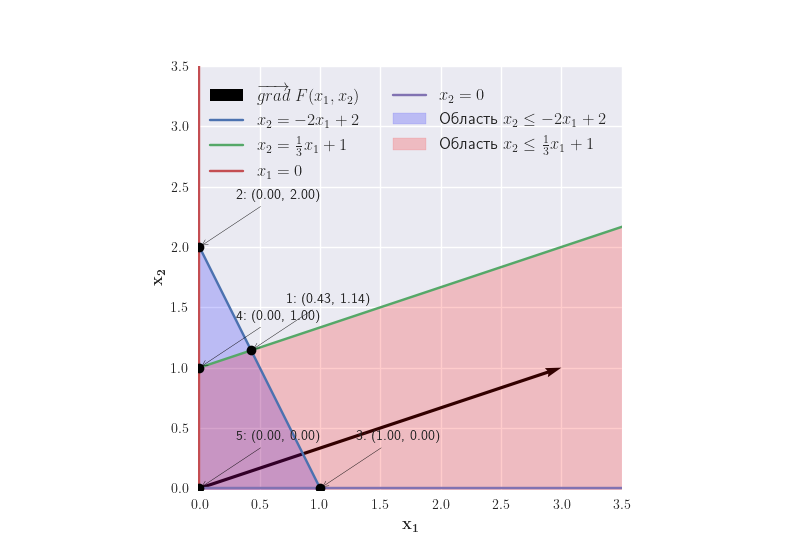
\includegraphics[width=1.0\textwidth]{images/01-lab/01-graphic.png}
    \caption{График к пункту А задания 1.}
    \label{01-lab-01-graphic}
\end{figure}

В условную область попадают все точки, кроме второй. Подставим подходящие точки в функцию $F$ и выведем её значения в этих точках:

\begin{lstlisting}[language=text]
    Значение F в точке 1 равно 2.43
    Значение F в точке 3 равно 3.00
    Значение F в точке 4 равно 1.00
    Значение F в точке 5 равно 0.00
\end{lstlisting}

\textbf{Ответ:} $\max F(x_1, x_2) = 3, \argmax F(x_1, x_2) = (1, 0);\\
    \min F(x_1, x_2) = 0, \argmin F(x_1, x_2) = (0, 0)$ \label{01-lab-a-answer}

\subsubsection{Пункт Б}\label{01-lab-b}

Приведем неравенство к наглядному виду:

\[
    \begin{cases}
        x_2 \geq \dfrac{1}{3} x_1 - \dfrac{2}{3} \\
        x_2 \geq -x_1 + 10                       \\
        x_1 \geq 0                               \\
        x_2 \geq 0
    \end{cases}
\]

\href{https://github.com/retrobannerS/optimization_methods/blob/main/python/01-lab/B.%2001.py}{Код для построения графика}. Его вывод:

\begin{figure}[H]
    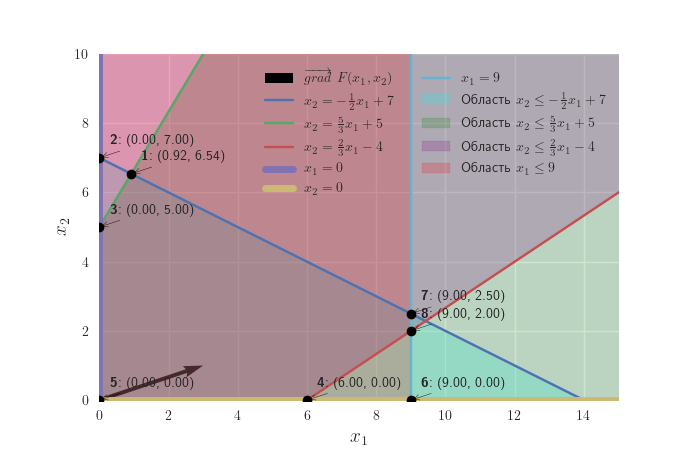
\includegraphics[width=1\textwidth, center]{images/01-lab/02-graphic.png}
    \caption{График к пункту Б задания 1.}
    \label{01-lab-02-graphic}
\end{figure}

Условная область неограничена. Градиент функции направлен внутрь первой четверти. Функция $F$ неограничена сверху. Её максимума не существует.

Осталось найти минимум $F$. Подходящие точки под номерами 1 и 3. Подставим подходящие точки в функцию $F$ и найдём её $min$:

\begin{lstlisting}[language=text]
    Значение F в точке 1 равно 26.00
    Значение F в точке 3 равно 10.00
\end{lstlisting}

\textbf{Ответ:} $\max F(x_1, x_2) \notin \R, \argmax F(x_1, x_2) \notin \R^2,\\
    \min F(x_1, x_2) = 10, \argmin F(x_1, x_2) = (0, 10)$ \label{01-lab-b-answer}

\subsubsection{Пункт В}\label{01-lab-c}

Приведем неравенство к более наглядному виду:
\[
    \begin{cases}
        x_2 \geq x_1 + 11            \\
        x_2 \leq \dfrac{1}{4}x_1 - 2 \\
        x_1 \geq 0                   \\
        x_2 \geq 0
    \end{cases}
\]

\href{https://github.com/retrobannerS/optimization_methods/blob/main/python/01-lab/C.%2001.py}{Код для построения графика}. Его вывод:

\begin{figure}[H]
    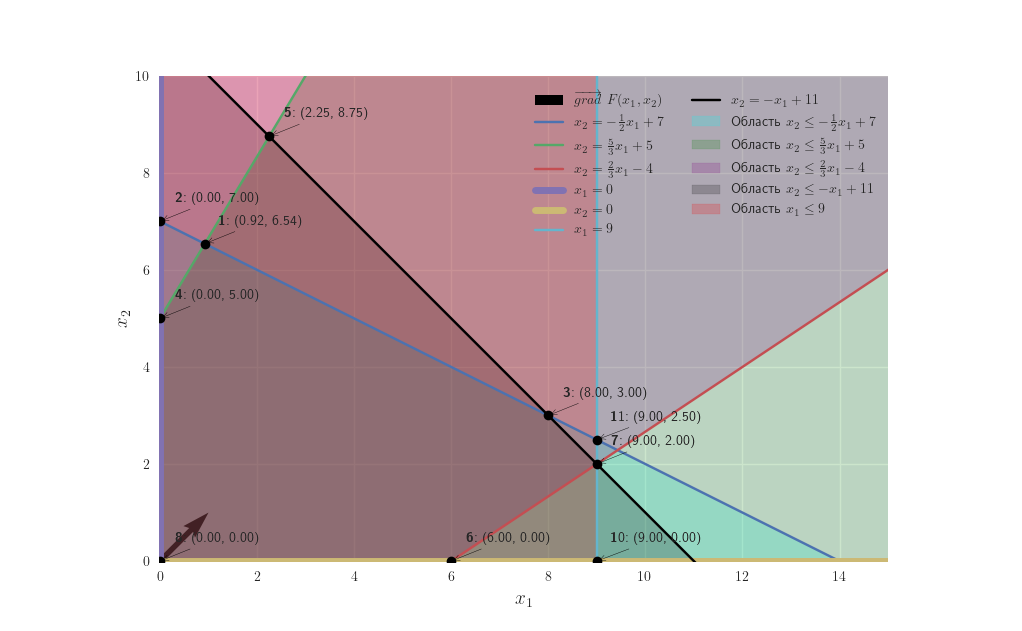
\includegraphics[width=1\textwidth, center]{images/01-lab/03-graphic.png}
    \caption{График к пункту В задания 1.}
    \label{01-lab-03-graphic}
\end{figure}

Как видно, мы имеем пустую условную область: $D = \varnothing$. Значит и $F(D) = \varnothing$. Максимума и минимума не существует.

\textbf{Ответ:} $\nexists\max F(x_1, x_2), \nexists\argmax F(x_1, x_2), \nexists\min F(x_1, x_2), \nexists\argmin F(x_1, x_2)$ \label{01-lab-c-answer}

\newpage

